\subsubsection{Scopo}
Include le attività e i compiti svolti per creare il \gl{prodotto}.
\subsubsection{Aspettative}
Le aspettative della corretta implementazione del processo sono:
\begin{itemize}
		\item realizzare un \gl{prodotto} finale conforme alle richieste del \gl{proponente} e che soddisfi le attività di \gl{validazione} e \gl{verifica};
		\item fissare gli obiettivi di sviluppo;
		\item fissare i vincoli tecnologici.
\end{itemize}

\subsubsection{Descrizione}
In accordo con lo standard \iso{ISO/IEC 12207}, il processo di sviluppo è composto dalle attività di:
\begin{itemize}
		\item analisi dei requisiti;
		\item progettazione;
		\item codifica;
		\item validazione.
\end{itemize}

\subsubsection{Analisi dei requisiti}
 \paragraph{Scopo dell'attività}
  Individuare i requisiti del \gl{progetto} dalle specifiche del \gl{capitolato} e tramite incontri con il pro-
  ponente. Tale attività produrrà un documento redatto dagli analisti, i quali avranno cura di elencare i \gl{casi d'uso} e i requisiti. Tale documento permette di
 capire le scelte di progettazione effettuate.
 \paragraph{Aspettative dell'attività}
 L'attività fissa come scopo la creazione di un documento che elencherà e rappresenterà i requisiti richiesti dal \gl{proponente}.
 \paragraph{Descrizione dell'attività}
 Tutti i requisiti analizzati, utilizzando le specifiche del \gl{capitolato} e consultando i proponenti negli
incontri effettuati, vanno specificati nell'\ARdocRR. Per analizzare e trovare i
requisiti si utilizza la tecnica dei \gl{casi d'uso}. Il tracciamento dei requisiti avviene tramite l'applicativo PragmaDB.
 \paragraph{Studio di fattibilità}
 Il \RESP{} di \gl{progetto} deve organizzare delle riunioni preventive, per permettere lo scambio
di opinioni tra i membri del gruppo sui capitolati proposti. Il documento \gl{prodotto} da queste
riunioni è lo \SFdocRR , il quale viene realizzato dagli \ANP{}. Essi devono
descrivere i seguenti punti: 
\begin{itemize}
 \item \textbf{Dominio tecnologico e applicativo}: si dà una valutazione prendendo in   considerazione
 la conoscenza attuale delle tecnologie richieste dal \gl{capitolato} in analisi da parte dei membri  
del gruppo;
 \item \textbf{Interesse strategico}: si valuta l'interesse strategico del gruppo di \gl{progetto} in relazione
al \gl{capitolato} in analisi;
 \item \textbf{Individuazione dei rischi}: si analizzano i possibili rischi in cui si può incorrere nel
\gl{capitolato} in analisi.
\end{itemize}
 \paragraph{\gl{Casi d'uso}}
 Ogni caso d'uso è così composto:
 \begin{itemize}
  \item \textbf{Codice identificativo}: codice univoco del caso d'uso in esame;
  \item \textbf{Titolo}: indica il titolo del caso d'uso;
  \item \textbf{Diagramma \gl{UML}}: rappresenta graficamente il caso d'uso;
  \item \textbf{Attori primari}: indica gli attori primari coinvolti;
  \item \textbf{Descrizione}: chiara, precisa e concisa descrizione del caso d'uso;
  \item \textbf{Precondizione}: indica la situazione che deve essere vera prima dell'esecuzione del caso d'uso;
  \item \textbf{Postcondizione} indica la situazione che deve essere vera dopo l'esecuzione del caso d'uso;
  \item \textbf{Scenario principale}: descrizione composta dal flusso dei \gl{casi d'uso} figli;
  \item \textbf{Scenari alternativi}: descrizione composta dai \gl{casi d'uso} che non appartengono al flusso
principale di esecuzione.
 \end{itemize}
 \paragraph{Codice identificativo dei \gl{casi d'uso}}
Ogni caso d'uso ha un proprio codice identificativo  che rispetta il seguente formalismo:\\ \\
\centerline{UC\textbraceleft{Codice}\textbraceright{}}
\\ \\dove:
\begin{itemize}
	\item \textbf{Codice}: indica il codice identificativo del requisito, è univoco e deve essere identificato in forma gerarchica.
\end{itemize}
 \paragraph{Requisiti}
 Ogni requisito è così composto:
  \begin{itemize}
  \item \textbf{Codice identificativo}: codice univoco del requisito;
  \item \textbf{Descrizione}: una breve descrizione, deve essere meno ambigua possibile;
  \item \textbf{Fonti}: identifica la fonte dalla quale è stato identificato il requisito.
 \end{itemize}
 \paragraph{Codice identificativo dei requisiti}
 Ogni requisito individuato avrà un codice identificativo univoco così formato: \\ \\
 \centerline{R\textbraceleft{}Tipo\textbraceright{}\textbraceleft{}Importanza\textbraceright{}\textbraceleft{}Codice\textbraceright{}}
 \\ \\
 dove:
 \begin{itemize}
 	\item \textbf{Tipo}: può assumere uno di questi valori:
 	\begin{itemize}
 		\item \textbf{F}: indica un requisito funzionale;
 		\item \textbf{Q}: indica un requisito di qualità;
 		\item \textbf{P}: indica un requisito prestazionale;
 		\item \textbf{V}: indica un requisito di vincolo.
 	\end{itemize}
 	\item \textbf{Importanza}: può assumere uno di questi valori:
 	\begin{itemize}
 		\item \textbf{O}: indica un requisito obbligatorio;
 		\item \textbf{D}: indica un requisito desiderabile;
 		\item \textbf{F}: indica un requisito facoltativo.
 	\end{itemize}
 	\item \textbf{Codice}: indica il codice identificativo del requisito, è univoco e deve essere identificato in forma gerarchica.
 \end{itemize}
 \paragraph{\gl{UML}}
 Viene utilizzata la versione corrente alla stesura del documento, ovvero la 2.5.

\subsubsection{Progettazione}
 \paragraph{Scopo dell'attività}
L'attività di progettazione definisce le linee essenziali della struttura del \gl{prodotto} \gl{software} in
funzione dei requisiti individuati dall'analisi. L'obiettivo del processo consiste nella stesura dei
documenti: \textit{"Specifica Tecnica"} e \textit{"Definizione di \gl{Prodotto}"}.
 \paragraph{Aspettative dell'attività}
Il processo porta alla formazione dei documenti sopracitati, i quali garantiscono affidabilità e
coerenza.
 \paragraph{Descrizione dell'attività}
La progettazione deve rispettare tutti i vincoli e i requisiti concordati tra i componenti del gruppo
e i proponenti. I documenti derivati da questa attività sono:
\begin{itemize}
	\item \textbf{Specifica tecnica}: descrive la progettazione ad alto livello relativa all'architettura dell'applicazione
e dei singoli componenti. Il documento specifica i diagrammi \gl{UML} ed i design
pattern utilizzati per realizzare l'architettura definendo inoltre i test necessari alla \gl{verifica};
	\item \textbf{Definizione di \gl{prodotto}}: descrive in dettaglio la progettazione di \gl{sistema}, integrando
quanto scritto nella Specifica Tecnica. Il documento specifica i diagrammi \gl{UML} e le
definizioni delle classi definendo inoltre i test necessari alla \gl{verifica}.
\end{itemize}
 \paragraph{Specifica tecnica}
\begin{itemize} 
	\item \textbf{Diagrammi \gl{UML}}:
	\begin{itemize}
	\item diagrammi delle classi;
	\item diagrammi dei \gl{package};
	\item diagrammi di attività;
	\item diagrammi di sequenza.
	\end{itemize}
	\item \textbf{\gl{Design pattern}}: devono essere descritti i \gl{design pattern} utilizzati per realizzare l'architettura. Ogni design
pattern deve essere accompagnato da una descrizione ed un diagramma, che ne esponga il
significato e la struttura;
	\item \textbf{Tracciamento delle componenti}:
	\item \textbf{Test di integrazione}: devono essere definite delle classi di \gl{verifica}, utili a verificare che ogni componente del
\gl{sistema} funzioni nella maniera appropriata.
\end{itemize}
 \paragraph{Definizione di \gl{prodotto}}
\begin{itemize}
	\item \textbf{Diagrammi \gl{UML}}:
	\begin{itemize}
		\item diagrammi delle classi;
		\item diagrammi di attività;
		\item diagrammi di sequenza.
	\end{itemize}
	\item \textbf{Definizioni delle classi}: ogni classe progettata deve essere descritta in modo da spiegarne lo scopo e definirne le
funzionalità ad essa associate.
	\item \textbf{Tracciamento delle classi}: ogni requisito deve essere tracciato, in modo da poter risalire alle classi ad esso associate. 
	\item \textbf{Test di unità}: devono essere definiti dei test di unità utili a verificare che le componenti del \gl{sistema} funzionino nel modo previsto.
\end{itemize}

\subsubsection{Codifica}
 \paragraph{Scopo dell'attività}
 Lo scopo dell'attività è l'implementazione del \gl{prodotto}, concretizzando la soluzione tramite la codifica.  
 \paragraph{Aspettative dell'attività}
 L'aspettativa dell'attività è un \gl{prodotto} corretto, ovvero stabile, affidabile, funzionale e che soddisfi i requisiti. 
 \paragraph{Descrizione dell'attività}
 L'attività deve rispettare i compiti e gli strumenti espressi nel \PPdocRR.
 \paragraph{Stile}
Le norme di stile saranno specificate in versioni successive di questo documento.
 \paragraph{Versionamento}
 Lo stile di rappresentazione della versione del codice verrà trattato e descritto in versioni successive di questo documento.
 \paragraph{\gl{Ricorsione}}
 La \gl{ricorsione} va evitata. Se non risulta accettabile convertirla in \gl{iterazione}, bisogna fornirne la prova di terminazione e l'analisi del costo in termini di spazio.
\subsubsection{Strumenti}
 \paragraph{PragmaDB} 
  PragmaDB è uno strumento open source di tracciamento dei requisiti. Verrà quindi utilizzato per semplificare e automatizzare il più possibile l'attività di analisi dei requisiti. In particolare, una volta inseriti casi d'uso, attori, requisiti e relative fonti, PragmaDB genera: 
  \begin{itemize}
  \item il codice \LaTeX{} relativo a casi d'uso e requisiti in forma tabellare;
  \item i diagrammi UML associati ai casi d'uso.
  \end{itemize}
  Essendo open source, questo strumento è stato adattato dal team \GRUPPO{} in base alle proprie necessità.
  \paragraph{\gl{Astah}}
  \gl{Astah} è uno strumento di modellazione \gl{UML}. Qualora i diagrammi UML generati da PragmaDB non siano soddisfacenti, si ricorrerà all'utilizzo di Astah. Viene utilizzata la versione 7.0 o superiori.
\begin{figure}[h]
\centering
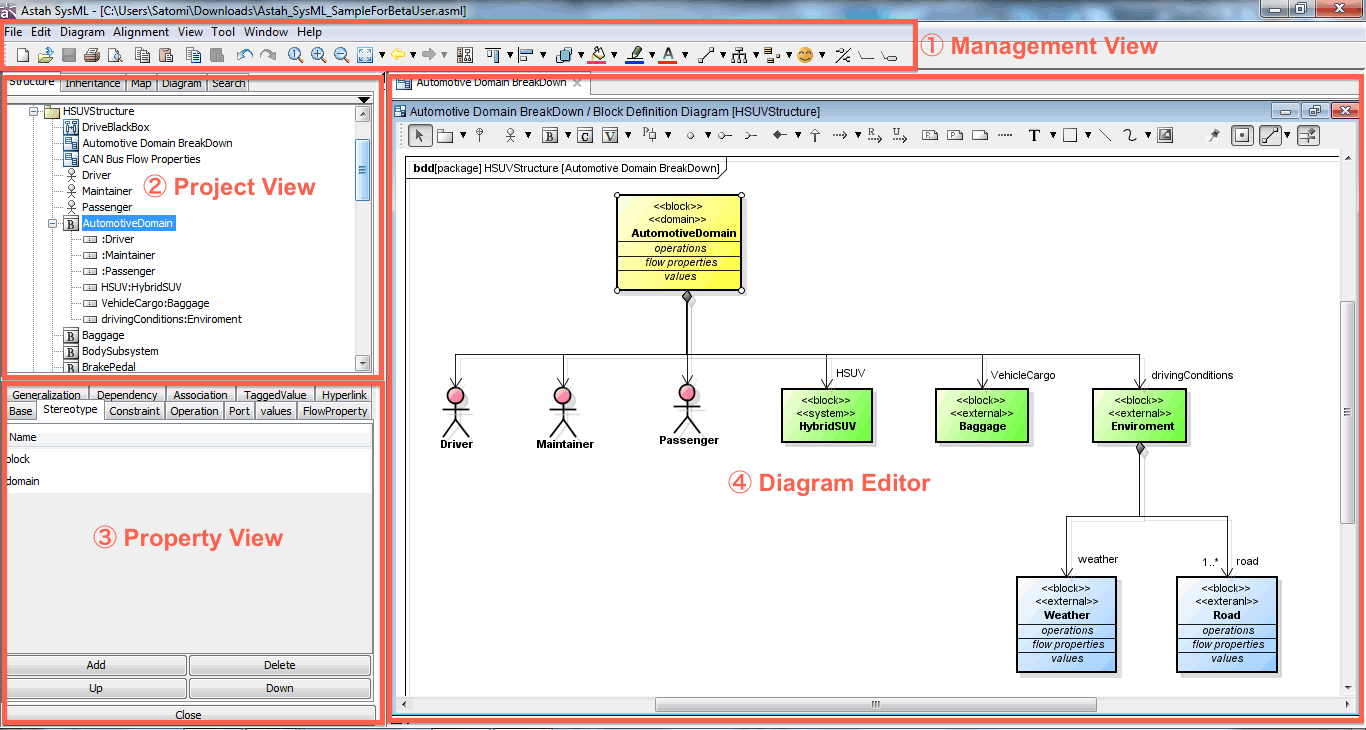
\includegraphics[scale=0.3]{img/astah.png}
\caption{Astah}\label{sec:Figura1}
\end{figure}

\newpage


  
